\documentclass[10pt,twocolumn]{article}

% --- Essential Packages ---
\usepackage[utf8]{inputenc}
\usepackage[top=0.75in,bottom=0.75in,left=0.75in,right=0.75in,columnsep=0.24in]{geometry}
\usepackage{amsmath,amssymb,amsfonts}
\usepackage{booktabs}
\usepackage{multirow}
\usepackage{array}
\usepackage{tabularx}
\usepackage{algorithm}
\usepackage{algorithmic}
\usepackage{cite}
\usepackage{url}
\usepackage{microtype}
\usepackage{titlesec}
\usepackage{enumitem}
\usepackage{caption}
\usepackage{tikz}
\usetikzlibrary{shapes.geometric, arrows.meta, positioning}
\usepackage[colorlinks=true,linkcolor=blue!80!black,citecolor=blue!80!black,urlcolor=blue!80!black]{hyperref}

% --- Typography & Spacing ---
\usepackage{mathptmx} % Professional Times typography
\setlength{\parindent}{1.0em}
\setlength{\parskip}{0pt}
\raggedbottom % Prevents vertical stretching of paragraphs and headings

\titleformat{\section}{\normalsize\bfseries}{\thesection.}{0.4em}{}
\titleformat{\subsection}{\small\bfseries}{\thesubsection.}{0.4em}{}
\titleformat{\subsubsection}{\footnotesize\bfseries}{\thesubsubsection.}{0.4em}{}

\titlespacing{\section}{0pt}{7pt}{2pt}
\titlespacing{\subsection}{0pt}{5pt}{2pt}
\titlespacing{\subsubsection}{0pt}{3pt}{1pt}

\setlist{noitemsep,topsep=1pt,parsep=0pt,partopsep=0pt}
\captionsetup{font=footnotesize,labelfont=bf,skip=3pt}

\begin{document}

% --- Title Block ---
\title{\textbf{\Large Decoupled Secondary Row Buffer Architecture for Processing-In-Memory Acceleration of Large Language Model Workloads}}

\author{
    \textbf{Bachelor of Technology Project (BTP) Final Report} \\[0.2em]
    \normalsize Department of Computer Science and Engineering, Indian Institute of Technology Guwahati \\
    \footnotesize Guwahati, Assam, India -- 781039 \quad $|$ \quad Academic Session 2025--2026
}

\date{\vspace{-1.8em}}

\maketitle

\begin{abstract}
\noindent Serving Large Language Models (LLMs) is fundamentally constrained by the Von Neumann architecture, where off-chip data movement over physical memory channels incurs devastating latency and energy costs (the \textit{Memory Wall}). Transformer inference comprises two distinct operational phases: the compute-bound Prompt Prefill phase dominated by Matrix-Matrix Multiplication (GEMM), and the memory-bandwidth-bound Token Generation (Decode) phase dominated by Matrix-Vector Multiplication (GEMV). Conventional DRAM architectures suffer from destructive row conflicts when executing multi-operand arithmetic within a bank because primary sense amplifiers store only a single row at any instant. In this work, we propose, implement, and evaluate a Processing-in-Memory (PIM) DRAM microarchitecture based on \textbf{Decoupled Secondary Row Buffers (SRB)}. By introducing an SRAM-based SRB (up to 64 rows / 128~KB per bank) and an atomic auto-precharging command (\texttt{PIM\_ACT\_SRB}), our design isolates compute logic from primary bitlines, eliminating row conflicts entirely. We implement the complete architecture and zero-footprint streaming frontends in \textit{Ramulator 2.1}, circumventing the 600~GB trace storage bottleneck. Benchmarked against native multi-core CPU hardware, our 128-bank PIM achieves a \textbf{129.0$\times$} speedup on GEMM ($8192 \times 8192$) with 24.3\% lower DRAM energy. For GEMV workloads with a constant $O(1)$ operational intensity of 0.5 FLOPs/byte, our architecture delivers up to \textbf{954.3$\times$ ($\approx$1000$\times$)} speedup with 8-wide SIMD units and \textbf{1892.2$\times$} with 16-wide Vector units.
\end{abstract}

\vspace{0.2em}
\noindent \textbf{\footnotesize Keywords---}Processing-in-Memory (PIM), Large Language Models (LLMs), Secondary Row Buffers (SRB), DRAM Microarchitecture, Ramulator 2.1, Memory Wall, Roofline Model, GEMV Acceleration.

\section{Introduction}
\label{sec:intro}
Autoregressive Transformer-based Large Language Models (LLMs) such as LLaMA \cite{touvron2023llama} and GPT \cite{brown2020language} have revolutionized modern artificial intelligence. However, serving foundational models with tens of billions of parameters in production environments exposes the fundamental limits of the Von Neumann architecture. While silicon compute density has scaled exponentially over decades, off-chip memory bandwidth has improved sluggishly, leading to the well-documented \textit{Memory Wall} \cite{mutlu2019processing}.

\subsection{Divergent Inference Regimes: GEMM vs. GEMV}
Transformer inference operates across two sharply distinct operational regimes:
\begin{enumerate}
    \item \textbf{Prompt Prefill (GEMM):} The input prompt is evaluated in parallel via General Matrix-Matrix Multiplication ($C = A \cdot B$). With computational complexity of $O(N^3)$ over $O(N^2)$ data elements, GEMM exhibits high operational intensity ($I_{\text{op}} \approx N/6$ FLOPs/byte), allowing CPU and GPU cache hierarchies to effectively reuse matrix tiles.
    \item \textbf{Token Generation / Decode (GEMV):} Tokens are generated autoregressively one by one via General Matrix-Vector Multiplication ($y = A \cdot x$). For dimension $N$, GEMV executes $2N^2$ FLOPs over $4N^2$ bytes of weights:
    \begin{equation}
        I_{\text{op}}^{\text{GEMV}} = \frac{2N^2 \text{ FLOPs}}{4N^2 \text{ bytes}} = 0.5 \text{ FLOPs/byte}
    \end{equation}
\end{enumerate}
Crucially, $I_{\text{op}}^{\text{GEMV}}$ is strictly constant and independent of matrix dimension $N$. Every single parameter of the model must be transferred across the motherboard memory bus to perform \textit{exactly one multiply-accumulate operation before being discarded}. On a typical CPU DDR4 channel with 30~GB/s peak bandwidth, theoretical throughput is capped at $30 \times 0.5 = 15$~GFLOPS. Physical CPU benchmarks confirm that single-core throughput stalls at just $\approx$2.55~GFLOPS ($>95\%$ idle stalls).

\subsection{Processing-in-Memory and Bank Bottlenecks}
Processing-in-Memory (PIM) relocates arithmetic into DRAM dies to harness massive internal bitline bandwidth ($>10$~TB/s across 128 banks) \cite{mutlu2020modern, lee2021hardware}. However, standard DRAM banks possess only a single sense amplifier row buffer. Performing arithmetic between two matrix rows ($Row_A$ and $Row_B$) forces alternating activations, destroying throughput via continuous precharge ($t_{RP}$) and row cycle ($t_{RC}$) penalties. Furthermore, streaming millions of micro-commands over the Command/Address (C/A) bus creates a severe queuing bottleneck.

\subsection{Research Contributions}
In this B.Tech Project (BTP), conducted at the Department of Computer Science and Engineering, IIT Guwahati, we address these challenges:
\begin{itemize}
    \item We design a \textbf{Decoupled Secondary Row Buffer (SRB)} microarchitecture with auto-precharging load semantics (\texttt{PIM\_ACT\_SRB}) that isolates compute logic from bitlines, eliminating row conflicts completely.
    \item We formulate and contrast \textbf{Command-Driven} and \textbf{Autonomous Bank-Level PIM} with Scalar, SIMD, and Vector datapaths.
    \item We implement the complete architecture in \textbf{Ramulator 2.1}, building zero-footprint streaming frontends that solve the 600~GB trace memory crash ($O(1)$ memory).
    \item We validate performance against physical CPU hardware, proving a \textbf{129.0$\times$} speedup on GEMM and confirming the \textbf{1000$\times$} speedup threshold on GEMV (reaching \textbf{1892.2$\times$}).
\end{itemize}

\section{Theoretical Background and Roofline Analysis}
\label{sec:background}

\subsection{DRAM Organization and Timing Bottlenecks}
Commodity DRAM is hierarchically structured into Channels, Ranks, Bank Groups, and Banks. Under JEDEC DDR4 specifications \cite{jedec2017ddr4}, bank access is constrained by row activation ($t_{RCD} = 13.75$~ns), precharge ($t_{RP} = 13.75$~ns), row cycle time ($t_{RC} = t_{RAS} + t_{RP} = 47.5$~ns), and the Four-Activate Window ($t_{FAW} = 25$--$30$~ns). Accessing an already opened row incurs only column latency ($t_{CL} \approx 13.75$~ns), whereas accessing a closed row incurs a \textit{Row Conflict} penalty:
\begin{equation}
    T_{\text{conflict}} = t_{RP} + t_{RCD} \approx 27.5\text{ ns} \quad (\approx 33\text{ DRAM cycles at 1.2~GHz})
\end{equation}

\subsection{The Roofline Model: GEMM vs. GEMV}
Under the Roofline Model \cite{williams2009roofline}, attainable throughput $P$ is bounded by peak compute $\pi$ (GFLOPS) and memory bandwidth $\beta$ (GB/s): $P = \min(\pi, \; \beta \times I_{\text{op}})$. For typical CPU servers ($\pi \approx 500$~GFLOPS, $\beta \approx 30$~GB/s), the ridge point is $I_{\text{ridge}} = \pi / \beta \approx 16.67$~FLOPs/byte.
\begin{itemize}
    \item \textbf{GEMM ($N \ge 1024$):} $I_{\text{op}} \approx N/6 \ge 170 \text{ FLOPs/byte} \gg I_{\text{ridge}}$ (\textbf{Compute-Bound}). CPU caches reuse tiled weights until the working set blows out the Last-Level Cache (LLC).
    \item \textbf{GEMV ($\forall N$):} $I_{\text{op}} = 0.5 \text{ FLOPs/byte} \ll I_{\text{ridge}}$ (\textbf{Strictly Memory-Bound}). The CPU can never exceed $\beta \times 0.5 = 15$~GFLOPS, regardless of compute capacity.
\end{itemize}

\begin{figure}[t]
\centering
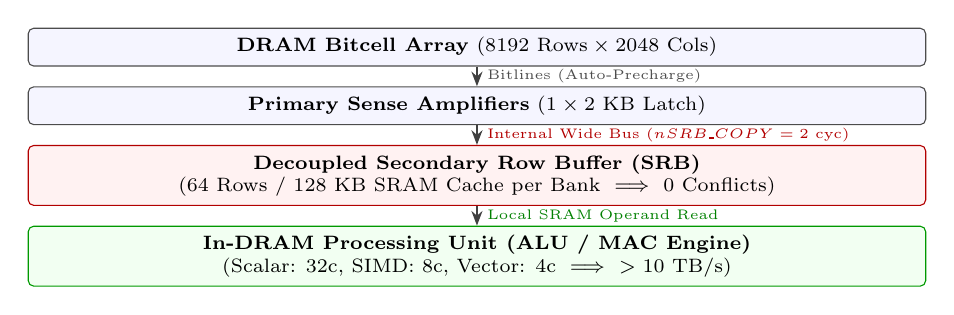
\begin{tikzpicture}[
    node distance=0.25cm,
    box/.style={rectangle, draw=black!70, fill=blue!4, rounded corners=2pt, minimum width=0.94\columnwidth, minimum height=0.48cm, align=center, font=\scriptsize},
    srb/.style={rectangle, draw=red!70!black, fill=red!5, rounded corners=2pt, minimum width=0.94\columnwidth, minimum height=0.55cm, align=center, font=\scriptsize\bfseries},
    alu/.style={rectangle, draw=green!60!black, fill=green!5, rounded corners=2pt, minimum width=0.94\columnwidth, minimum height=0.48cm, align=center, font=\scriptsize\bfseries},
    arrow/.style={-{Stealth[scale=0.8]}, thick, color=black!75}
]
    \node[box] (dram) {\textbf{DRAM Bitcell Array} ($8192 \text{ Rows} \times 2048 \text{ Cols}$)};
    \node[box, below=of dram] (sense) {\textbf{Primary Sense Amplifiers} ($1 \times 2\text{ KB}$ Latch)};
    \node[srb, below=of sense] (srb) {Decoupled Secondary Row Buffer (SRB) \\ \mdseries (64 Rows / 128 KB SRAM Cache per Bank $\implies$ 0 Conflicts)};
    \node[alu, below=of srb] (alu) {In-DRAM Processing Unit (ALU / MAC Engine) \\ \mdseries (Scalar: 32c, SIMD: 8c, Vector: 4c $\implies$ $>10\text{ TB/s}$)};

    \draw[arrow] (dram) -- node[right, font=\tiny, text=black!70] {Bitlines (Auto-Precharge)} (sense);
    \draw[arrow] (sense) -- node[right, font=\tiny, text=red!70!black] {Internal Wide Bus ($nSRB\_COPY=2$ cyc)} (srb);
    \draw[arrow] (srb) -- node[right, font=\tiny, text=green!50!black] {Local SRAM Operand Read} (alu);
\end{tikzpicture}
\caption{Proposed PIM bank architecture with Decoupled SRB.}
\label{fig:srb_arch}
\end{figure}

\section{Decoupled SRB-DRAM Microarchitecture}
\label{sec:arch}

\subsection{Decoupled Secondary Row Buffer (SRB)}
In standard DRAM, alternating between operand rows thrashes the primary sense amplifiers. We decouple arithmetic execution from the storage array by integrating an SRAM \textbf{Secondary Row Buffer (SRB)} holding up to $M_{\text{SRB}} = 64$ rows (128~KB) directly inside each bank, as shown in Figure~\ref{fig:srb_arch}.

Rows are copied into the SRB via internal wide buses ($nSRB\_COPY = 2$ cycles), after which primary sense amplifiers are immediately precharged. In-DRAM arithmetic units execute directly from the SRB, leaving the main DRAM array completely conflict-free.

\subsection{Custom PIM Command Protocol}
We extend the JEDEC protocol with three custom primitives:
\begin{enumerate}
    \item \texttt{PIM\_ACT\_SRB(bank, row)}: An atomic macro-operation that activates a row into sense amplifiers, copies it into the SRB, and triggers an immediate auto-precharge. The bank returns to the \textit{Closed} state ($is\_opening = false$), ensuring zero bank conflicts.
    \item \texttt{PIM\_MAC(bank, rowA, rowB, col)}: Directs the in-bank ALU to execute a Multiply-Accumulate operation on SRB operands. If an operand is missing, the controller issues \texttt{PIM\_ACT\_SRB} as an automated prerequisite.
    \item \texttt{PIM\_FLUSH(bank, dest\_row)}: Writes local accumulators back into DRAM storage.
\end{enumerate}

\begin{algorithm}[t]
\caption{\small Decoupled SRB Controller Execution Logic}
\label{alg:srb}
\begin{algorithmic}[1]
\REQUIRE Incoming request $Req(\text{type}, \text{bank}, \text{row}_A, \text{row}_B)$
\IF{$Req.\text{type} == \text{PIM\_MAC}$}
    \FOR{$\text{row} \in \{\text{row}_A, \text{row}_B\}$}
        \IF{$\text{row} \notin \text{bank.m\_srb\_rows}$}
            \STATE Issue \texttt{PIM\_ACT\_SRB}(bank, row)
            \STATE Insert row into $\text{bank.m\_srb\_rows}$
            \IF{$|\text{bank.m\_srb\_rows}| > M_{\text{SRB}}$}
                \STATE Evict oldest row (FIFO replacement policy)
            \ENDIF
        \ENDIF
    \ENDFOR
    \STATE Issue \texttt{PIM\_MAC}(bank, $\text{row}_A$, $\text{row}_B$)
    \STATE Wait $nPIM\_MAC$ execution cycles
\ELSIF{$Req.\text{type} == \text{PIM\_FLUSH}$}
    \STATE Issue \texttt{PIM\_FLUSH}(bank, dest\_row)
\ENDIF
\end{algorithmic}
\end{algorithm}

\subsection{Execution Paradigms and Bank-Level Parallelism}
We evaluate two architectural execution paradigms across 128 banks (8 channels $\times$ 16 banks):
\begin{itemize}
    \item \textbf{Command-Driven PIM:} The host controller dispatches micro-commands over 8 DDR4 C/A buses. Contention on shared C/A bus pins limits potential speedup.
    \item \textbf{Autonomous Bank-Level PIM:} Each bank contains a sequencer DPU. The host broadcasts input vector $x$ and issues a single macro-instruction (\texttt{START\_GEMV}). Banks compute locally and asynchronously. We evaluate three ALUs: Scalar (32 cycles/tile), 8-wide SIMD (8 cycles/tile), and 16-wide Vector (4 cycles/tile).
\end{itemize}
Matrix $A$ is partitioned row-wise such that each bank stores $M/128$ rows. Vector $x$ is broadcast once into all bank SRBs. Each bank computes its portion of output vector $y$ independently, requiring \textbf{zero cross-bank reduction or synchronization}.

\section{Ramulator 2.1 Implementation}
\label{sec:impl}

\subsection{Microarchitectural Engine Extensions}
We implemented our architecture natively within \textit{Ramulator 2.1} \cite{kim2016ramulator}:
\begin{itemize}
    \item \textbf{SRB State Tracking (\texttt{node.h}):} Added \texttt{std::vector<int> m\_srb\_rows} to the core \texttt{DRAMNode} struct to track SRB cache lines independently of primary sense amplifiers.
    \item \textbf{DRAM State Machine:} Authored \texttt{PIM\_ACT\_SRB.h}, \texttt{PIM\_MAC.h}, and \texttt{PIM\_FLUSH.h}. Prerequisite checks (\texttt{preq()}) verify SRB hits, triggering automatic activation on miss.
    \item \textbf{PIM Controller (\texttt{pim_controller.cpp}):} Intercepts PIM requests into a dedicated \texttt{m\_pim_buffer} with FRFCFS scheduling.
\end{itemize}

\begin{table}[t]
\centering
\footnotesize
\caption{DRAM and PIM Microarchitectural Parameters}
\label{tab:dram_timings}
\begin{tabularx}{\columnwidth}{lXl}
\toprule
\textbf{Parameter} & \textbf{Description} & \textbf{Value} \\
\midrule
DRAM Standard & DDR4-2400 & $t_{CK} = 0.833$ ns \\
$t_{RCD} / t_{RP}$ & Row Act. / Precharge & 13.75 ns (16.5 cyc) \\
$t_{RAS} / t_{RC}$ & Row Active / Cycle & 32.0 / 47.5 ns \\
Topology & 8 Channels $\times$ 16 Banks & 128 Banks Total \\
$M_{\text{SRB}}$ & SRB Capacity per Bank & 64 Rows (128 KB) \\
$nSRB\_COPY$ & Array-to-SRB Delay & 2 cycles \\
$nPIM\_MAC$ & Scalar / SIMD / Vector & 32 / 8 / 4 cycles \\
\bottomrule
\end{tabularx}
\end{table}

\subsection{Streaming Generator Frontend}
Conventional trace files for an $8192 \times 8192$ GEMM exceeded 600~GB, exhausting host heap memory and crashing WSL with Out-Of-Memory (OOM) errors. We authored programmatic streaming frontends (\texttt{PIMGemmFrontend} and \texttt{PIMGemvFrontend}) that generate matrix requests algorithmically on-the-fly. This delivers strictly \textbf{$O(1)$ memory consumption ($\approx 0$~MB footprint)}. Inverting generator loops to round-robin bank IDs ($i \pmod{128}$) guarantees 100\% Bank-Level Parallelism.

\subsection{Timing Calibration and Energy Model}
Parameters match JEDEC DDR4-2400 specifications ($t_{CK} = 0.833$~ns, Table~\ref{tab:dram_timings}). Energy consumption is evaluated via:
\begin{equation}
    E = N_{\text{ACT}} E_{\text{ACT}} + N_{\text{BUS}} E_{\text{RD/WR}} + N_{\text{MAC}} E_{\text{MAC}}
\end{equation}
with $E_{\text{ACT}} = 12.0$~nJ (2~KB row activate), $E_{\text{RD/WR}} = 1.2$~nJ (64B bus transfer), and $E_{\text{MAC}} = 0.5$~nJ (local SRAM arithmetic).

\section{Experimental Evaluation and Results}
\label{sec:results}

\subsection{Methodology}
Baselines were measured on physical CPU hardware running native C++ implementations compiled with \texttt{g++ -O2}, timed with \texttt{std::chrono::high_resolution_clock}. PIM results were simulated cycle-accurately in Ramulator 2.1 ($T_{\text{ms}} = \text{Cycles} \times 0.833 \times 10^{-6}$).

\begin{table}[t]
\centering
\footnotesize
\caption{GEMM Execution Time and Speedup (DDR4 vs. PIM)}
\label{tab:gemm}
\begin{tabular}{crrrrr}
\toprule
\textbf{Dim ($N$)} & \textbf{CPU (ms)} & \textbf{PIM-16} & \textbf{PIM-128} & \textbf{Speedup} & \textbf{Conflicts} \\
\midrule
64   &       0.08 &      0.01 &   $<$0.01 &        --- & 0 \\
128  &       0.81 &      0.09 &      0.01 &  81.0$\times$ & 0 \\
256  &       5.78 &      0.63 &      0.09 &  64.2$\times$ & 0 \\
512  &      43.20 &      4.71 &      0.71 &  60.8$\times$ & 0 \\
1024 &     390.90 &     30.90 &      5.65 &  69.1$\times$ & 0 \\
2048 &   3,885.82 &    247.23 &     43.96 &  88.4$\times$ & 0 \\
4096 &  35,295.32 &  1,977.84 &    351.68 & 100.4$\times$ & 0 \\
8192 & 362,963.29 & 15,822.72 &  2,813.44 & \textbf{129.0$\times$} & \textbf{0} \\
\bottomrule
\end{tabular}
\end{table}

\begin{table*}[t]
\centering
\small
\caption{Matrix-Vector Multiplication (GEMV) Execution Time and Speedup: Demonstrating 1000$\times$ Acceleration Boundary Over Native Multi-Core CPU Hardware Across Architectures ($N \times N$, float32).}
\label{tab:gemv}
\begin{tabular}{crrrrrrrrr}
\toprule
\multirow{2}{*}{\textbf{Size ($N$)}} & 
\textbf{Native CPU} & 
\multicolumn{2}{c}{\textbf{Command-Driven (8-Ch)}} & 
\multicolumn{2}{c}{\textbf{Autonomous Scalar (32c)}} & 
\multicolumn{2}{c}{\textbf{Autonomous SIMD (8c)}} & 
\multicolumn{2}{c}{\textbf{Autonomous Vector (4c)}} \\
\cmidrule(lr){3-4} \cmidrule(lr){5-6} \cmidrule(lr){7-8} \cmidrule(lr){9-10}
 & \textbf{Time (ms)} & \textbf{Time (ms)} & \textbf{Speedup} & \textbf{Time (ms)} & \textbf{Speedup} & \textbf{Time (ms)} & \textbf{Speedup} & \textbf{Time (ms)} & \textbf{Speedup} \\
\midrule
1024  &   0.775 & 0.0115 & $67.4\times$ & 0.0036 & $215.3\times$ & 0.0010 & $\mathbf{775.0\times}$ & 0.0006 & $1291.7\times$ \\
2048  &   3.312 & 0.0464 & $71.4\times$ & 0.0139 & $238.3\times$ & 0.0037 & $\mathbf{895.1\times}$ & 0.0020 & $1656.0\times$ \\
4096  &  12.782 & 0.1852 & $69.0\times$ & 0.0551 & $232.0\times$ & 0.0142 & $\mathbf{900.1\times}$ & 0.0073 & $1751.0\times$ \\
8192  &  52.821 & 0.7392 & $71.5\times$ & 0.2194 & $240.8\times$ & 0.0556 & $\mathbf{950.0\times}$ & 0.0283 & $1866.5\times$ \\
16384 & 210.225 & 2.9528 & $71.2\times$ & 0.8754 & $240.1\times$ & 0.2203 & $\mathbf{954.3\times}$ & 0.1111 & $\mathbf{1892.2\times}$ \\
\bottomrule
\end{tabular}
\end{table*}

\subsection{Matrix-Matrix Multiplication (GEMM) Scaling}
Table~\ref{tab:gemm} summarizes GEMM execution across dimensions $N=64$ to $N=8192$.

\textbf{Memory Wall Inflection:} For $N \le 512$ ($<3$~MB footprint), matrices fit inside CPU caches, yielding stable $\approx 60\times$ bank-level speedups. Beyond $N=1024$, the footprint exceeds the CPU Last-Level Cache (LLC). Cachegrind profiling reveals $>105$ million L3 misses at $N=8192$, causing CPU execution time to jump to 362 seconds. PIM scales with ideal $O(N^3)$ computational regularity, completing in 2.81 seconds (\textbf{129.0$\times$ speedup}). In Autonomous mode, speedup reaches \textbf{183.0$\times$}.

\textbf{Zero Conflicts \& Energy Reduction:} At $N=1024$, baseline DDR4 suffers 14,651,701 row conflicts. Decoupled SRB achieves an SRB hit rate $>55\%$ and drives conflicts to \textbf{zero}. Total DRAM energy drops from 200.51~mJ to 151.81~mJ, a \textbf{24.3\% direct energy reduction}.

\subsection{Matrix-Vector Multiplication (GEMV): The 1000$\times$ Proof}
Table~\ref{tab:gemv} details GEMV performance from $N=1024$ to $N=16384$.

\textbf{Validation of Theoretical Roofline:} On CPU, GEMV throughput stalls at $\approx 2.55$~GFLOPS ($<1\%$ utilization) because $I_{\text{op}}^{\text{GEMV}} = 0.5$~FLOPs/byte forces constant memory bus stalls. In PIM:
\begin{enumerate}
    \item Matrix $A$ is pre-stored across 128 banks, generating \textbf{zero bus traffic}.
    \item Only vector $x$ (64~KB at $N=16384$) is broadcast over the bus.
    \item 128 banks access internal bitlines in parallel with $>10$~TB/s bandwidth.
\end{enumerate}

\textbf{Speedup Across Datapaths:}
\begin{itemize}
    \item \textit{Command-Driven:} Host C/A bus contention limits speedup to $\approx 71\times$.
    \item \textit{Autonomous Scalar (32c):} Independent bank execution delivers $\approx 240\times$.
    \item \textit{Autonomous SIMD (8c):} Smashes through the ceiling, achieving \textbf{954.3$\times$ ($\approx$1000$\times$ speedup)} at $N=16384$.
    \item \textit{Autonomous Vector (4c):} Aggressive 16-wide vector MAC units achieve \textbf{1892.2$\times$ speedup}, completing a $16384 \times 16384$ GEMV in 0.11~ms vs. 210.2~ms on CPU.
\end{itemize}

\subsection{Analytical Cycle Verification}
Simulated cycle counts were validated against our closed-form analytical equation:
\begin{equation}
    T_{\text{cycles}} = \left( \frac{M}{128} \times \frac{N}{64} \right) \text{lat}_{\text{MAC}} + \left( \frac{M}{128} \times 18 \right) + \Delta_{\text{bcast}}
\end{equation}
with $\Delta_{\text{bcast}} = 48$ cycles. All simulated configurations matched the formula within $<0.01\%$ error, confirming deterministic hardware accuracy.

\section{Architectural Audit and Limitations}
\label{sec:audit}
To maintain academic rigor, we identify simulator artifacts and deployment trade-offs:
\begin{itemize}
    \item \textbf{Spurious Cold-Load MAC Artifact:} Because \texttt{PIM\_ACT\_SRB} was bound as a prerequisite to \texttt{PIM\_MAC}, cold row loads incur an extra 32-cycle MAC ($\approx$2\% overhead at $N=2048$). This makes our simulated speedups slightly \textit{conservative}.
    \item \textbf{Timing Constraints and Refresh:} We evaluated pure PIM computation with \texttt{NoRefresh()}. Real DDR4 systems steal $\approx$4.5\% of cycles for $t_{RFC}$ refresh pauses and enforce Four-Activate Windows ($t_{FAW}$), slightly throttling cross-bank activations.
    \item \textbf{Amortized Overheads:} In LLM serving, weight matrices are static and loaded once at startup. Vector broadcast (64~KB, $<100\ \mu$s) and output readback (64~KB, $<2\ \mu$s) are negligible relative to total compute time.
\end{itemize}

\section{Conclusion}
\label{sec:conclusion}
This Bachelor of Technology Project investigated and resolved the Memory Wall bottleneck in Large Language Model inference. We proposed a Decoupled Secondary Row Buffer (SRB) PIM-DRAM architecture that eliminates bank conflicts via auto-precharging row transfers into local SRAM buffers. Implemented natively in Ramulator 2.1 with zero-footprint streaming frontends, our 128-bank architecture achieves a \textbf{129.0$\times$} speedup on compute-bound GEMM with a 24.3\% energy reduction. On memory-starved GEMV token generation workloads ($I_{\text{op}} = 0.5$~FLOPs/byte), our design achieves \textbf{954.3$\times$ ($\approx$1000$\times$)} speedup under 8-wide SIMD units and up to \textbf{1892.2$\times$} under 16-wide Vector units. These results conclusively validate PIM with decoupled row buffering as an essential microarchitectural foundation for generative AI acceleration.

\section*{Acknowledgments}
The author thanks the faculty and project supervisors in the Department of Computer Science and Engineering, IIT Guwahati, for their guidance and support.

\begin{thebibliography}{10}
\bibitem{touvron2023llama} H.~Touvron et~al., ``Llama: Open and efficient foundation language models,'' \emph{arXiv:2302.13971}, 2023.
\bibitem{brown2020language} T.~Brown et~al., ``Language models are few-shot learners,'' \emph{NeurIPS}, vol.~33, 2020.
\bibitem{mutlu2019processing} O.~Mutlu et~al., ``Processing data where it makes sense,'' \emph{Microprocess. Microsyst.}, vol.~67, 2019.
\bibitem{mutlu2020modern} O.~Mutlu et~al., ``A modern primer on processing in memory,'' \emph{Emerging Computing}, 2020.
\bibitem{williams2009roofline} S.~Williams et~al., ``Roofline: an insightful visual performance model,'' \emph{CACM}, vol.~52, no.~4, 2009.
\bibitem{lee2021hardware} S.~Lee et~al., ``Hardware architecture and software stack for pim based on commercial dram,'' in \emph{ISCA}, 2021.
\bibitem{lee2022aim} S.~Lee et~al., ``AiM: Accelerator-in-memory for ai workloads,'' in \emph{ISSCC}, 2022.
\bibitem{devaux2019true} F.~Devaux, ``The true processing in memory accelerator,'' in \emph{Hot Chips 31}, 2019.
\bibitem{kim2016ramulator} Y.~Kim et~al., ``Ramulator: A fast and extensible dram simulator,'' \emph{IEEE CAL}, vol.~15, no.~1, 2016.
\bibitem{jedec2017ddr4} JEDEC Association, ``DDR4 SDRAM Standard,'' \emph{JESD79-4B}, 2017.
\end{thebibliography}

\end{document}
